% ============================================================
% content/questions.tex —— 2020 全国Ⅰ卷（理综物理部分）· 试题
% 来源：2020/2020_物理真题_含解析.md（物理备课大师 Word 版转录）
% 题号保留官方编号 14--25、33--34；第 1--13 题为理综其他科目。
% 图形见 figures/（全部为 TikZ/circuitikz/pgfplots 矢量重绘）
% ============================================================

\begin{gknotice}
  \textbf{卷种说明：}本卷为 2020 年普通高等学校招生全国统一考试理科综合能力测试（全国卷Ⅰ）的物理部分，
  满分 110 分，考试用时 90 分钟，共 14 小题。选择题题号从 14 开始，因为第 1--13 题为理综其他科目试题，
  本工程只收录物理部分。第 33、34 题为选考题（选修 3-3、选修 3-4），考生按原卷要求任选一题作答。
\end{gknotice}

\gkpart{二、选择题}

\textbf{（本题共 8 小题，每小题 6 分，共 48 分。在每小题给出的四个选项中，第 14--18 题只有一项符合题目要求，第 19--21 题有多项符合题目要求。全部选对的得 6 分，选对但不全的得 3 分，有选错的得 0 分。）}

\begin{question}
\gkti{14}行驶中的汽车如果发生剧烈碰撞，车内的安全气囊会被弹出并瞬间充满气体。若碰撞后汽车的速度在很短时间内减小为零，关于安全气囊在此过程中的作用，下列说法正确的是\gkblank

\begin{gkopts}(1)
  \task A．增加了司机单位面积的受力大小
  \task B．减少了碰撞前后司机动量的变化量
  \task C．将司机的动能全部转换成汽车的动能
  \task D．延长了司机的受力时间并增大了司机的受力面积
\end{gkopts}
\end{question}

\begin{question}
\gkti{15}火星的质量约为地球质量的 $\dfrac{1}{10}$，半径约为地球半径的 $\dfrac{1}{2}$，则同一物体在火星表面与在地球表面受到的引力的比值约为\gkblank

\begin{gkopts}(4)
  \task A．$0.2$
  \task B．$0.4$
  \task C．$2.0$
  \task D．$2.5$
\end{gkopts}
\end{question}

\begin{question}
\gkti{16}如图所示，一同学表演荡秋千。已知秋千的两根绳长均为 \SI{10}{\metre}，该同学和秋千踏板的总质量约为 \SI{50}{\kilogram}。绳的质量忽略不计。当该同学荡到秋千支架的正下方时，速度大小为 \SI{8}{\metre\per\second}，此时每根绳子平均承受的拉力约为\gkblank

\gkfig{figures/q16-swing}

\begin{gkopts}(4)
  \task A．\SI{200}{\newton}
  \task B．\SI{400}{\newton}
  \task C．\SI{600}{\newton}
  \task D．\SI{800}{\newton}
\end{gkopts}
\end{question}

\begin{question}
\gkti{17}图甲所示的电路中，$K$ 与 $L$ 间接一智能电源，用以控制电容器 $C$ 两端的电压 $U_C$。如果 $U_C$ 随时间 $t$ 的变化如图乙所示，则下列描述电阻 $R$ 两端电压 $U_R$ 随时间 $t$ 变化的图像中，正确的是\gkblank

\gkfig{figures/q17-figure}

\begin{gkopts}(2)
  \task A．% 第 17 题选项 A：U_R 在 0--1 s 为 0，1--2 s 为 +U，2--3 s 为 0，3--5 s 为 -U/2
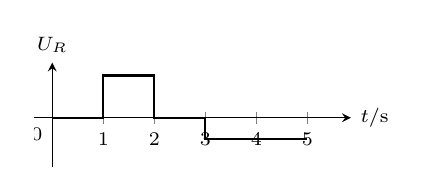
\begin{tikzpicture}
  \begin{axis}[
      width=5.6cm, height=2.9cm,
      axis lines=middle,
      xmin=-0.35, xmax=5.85, ymin=-1.15, ymax=1.3,
      xtick={1,2,3,4,5}, ytick=\empty,
      xlabel={$t$/s}, ylabel={$U_R$},
      xlabel style={anchor=west}, ylabel style={anchor=south},
      tick label style={font=\scriptsize}, label style={font=\scriptsize},
      font=\scriptsize]
    \addplot[thick, const plot] coordinates
      {(0,0) (1,0) (1,1) (2,1) (2,0) (3,0) (3,-0.5) (5,-0.5)};
    \node[below left] at (axis cs:0,0) {$0$};
  \end{axis}
\end{tikzpicture}

  \task B．% 第 17 题选项 B：0--1 s 为 0，1--2 s 为 +U，2--3 s 为 0，3--5 s 为 +U/2
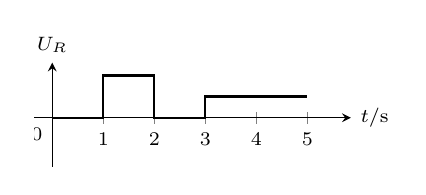
\begin{tikzpicture}
  \begin{axis}[
      width=5.6cm, height=2.9cm,
      axis lines=middle,
      xmin=-0.35, xmax=5.85, ymin=-1.15, ymax=1.3,
      xtick={1,2,3,4,5}, ytick=\empty,
      xlabel={$t$/s}, ylabel={$U_R$},
      xlabel style={anchor=west}, ylabel style={anchor=south},
      tick label style={font=\scriptsize}, label style={font=\scriptsize},
      font=\scriptsize]
    \addplot[thick, const plot] coordinates
      {(0,0) (1,0) (1,1) (2,1) (2,0) (3,0) (3,0.5) (5,0.5)};
    \node[below left] at (axis cs:0,0) {$0$};
  \end{axis}
\end{tikzpicture}

  \task C．% 第 17 题选项 C：0--1 s 为 0，1--2 s 为 +U，2--3 s 为 0，3--5 s 为 -U
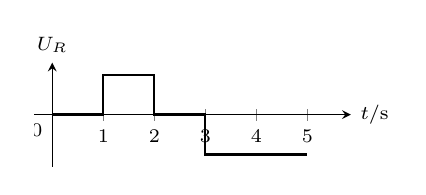
\begin{tikzpicture}
  \begin{axis}[
      width=5.6cm, height=2.9cm,
      axis lines=middle,
      xmin=-0.35, xmax=5.85, ymin=-1.3, ymax=1.3,
      xtick={1,2,3,4,5}, ytick=\empty,
      xlabel={$t$/s}, ylabel={$U_R$},
      xlabel style={anchor=west}, ylabel style={anchor=south},
      tick label style={font=\scriptsize}, label style={font=\scriptsize},
      font=\scriptsize]
    \addplot[thick, const plot] coordinates
      {(0,0) (1,0) (1,1) (2,1) (2,0) (3,0) (3,-1) (5,-1)};
    \node[below left] at (axis cs:0,0) {$0$};
  \end{axis}
\end{tikzpicture}

  \task D．% 第 17 题选项 D：0--1 s 为 0，1--2 s 线性升至 +U，2--3 s 保持，3--5 s 线性降为 0
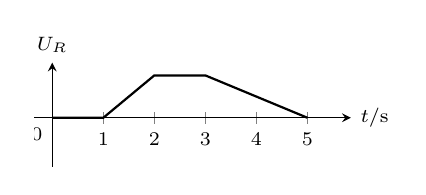
\begin{tikzpicture}
  \begin{axis}[
      width=5.6cm, height=2.9cm,
      axis lines=middle,
      xmin=-0.35, xmax=5.85, ymin=-1.15, ymax=1.3,
      xtick={1,2,3,4,5}, ytick=\empty,
      xlabel={$t$/s}, ylabel={$U_R$},
      xlabel style={anchor=west}, ylabel style={anchor=south},
      tick label style={font=\scriptsize}, label style={font=\scriptsize},
      font=\scriptsize]
    \addplot[thick] coordinates {(0,0) (1,0) (2,1) (3,1) (5,0)};
    \node[below left] at (axis cs:0,0) {$0$};
  \end{axis}
\end{tikzpicture}

\end{gkopts}
\end{question}

\begin{question}
\gkti{18}一匀强磁场的磁感应强度大小为 $B$，方向垂直于纸面向外，其边界如图中虚线所示，$\overset{\frown}{ab}$ 为半圆，$ac$、$bd$ 与直径 $ab$ 共线，$ac$ 间的距离等于半圆的半径。一束质量为 $m$、电荷量为 $q$（$q>0$）的粒子，在纸面内从 $c$ 点垂直于 $ac$ 射入磁场，这些粒子具有各种速率。不计粒子之间的相互作用。在磁场中运动时间最长的粒子，其运动时间为\gkblank

\gkfig{figures/q18-field}

\begin{gkopts}(4)
  \task A．$\dfrac{7\pi m}{6qB}$
  \task B．$\dfrac{5\pi m}{4qB}$
  \task C．$\dfrac{4\pi m}{3qB}$
  \task D．$\dfrac{3\pi m}{2qB}$
\end{gkopts}
\end{question}

\begin{question}
\gkti{19}下列核反应方程中，$\mathrm{X}_1$、$\mathrm{X}_2$、$\mathrm{X}_3$、$\mathrm{X}_4$ 代表 $\alpha$ 粒子的有\gkblank

\begin{gkopts}(1)
  \task A．${}_{1}^{2}\mathrm{H}+{}_{1}^{2}\mathrm{H}\to{}_{0}^{1}\mathrm{n}+\mathrm{X}_1$
  \task B．${}_{1}^{2}\mathrm{H}+{}_{1}^{3}\mathrm{H}\to{}_{0}^{1}\mathrm{n}+\mathrm{X}_2$
  \task C．${}_{92}^{235}\mathrm{U}+{}_{0}^{1}\mathrm{n}\to{}_{56}^{144}\mathrm{Ba}+{}_{36}^{89}\mathrm{Kr}+3\mathrm{X}_3$
  \task D．${}_{0}^{1}\mathrm{n}+{}_{3}^{6}\mathrm{Li}\to{}_{1}^{3}\mathrm{H}+\mathrm{X}_4$
\end{gkopts}
\end{question}

\begin{question}
\gkti{20}一物块在高 \SI{3.0}{\metre}、长 \SI{5.0}{\metre} 的斜面顶端从静止开始沿斜面下滑，其重力势能和动能随下滑距离 $s$ 的变化如图中直线Ⅰ、Ⅱ所示，重力加速度取 \SI{10}{\metre\per\second\squared}。则\gkblank

\gkfig{figures/q20-energy}

\begin{gkopts}(2)
  \task A．物块下滑过程中机械能不守恒
  \task B．物块与斜面间的动摩擦因数为 $0.5$
  \task C．物块下滑时加速度的大小为 \SI{6.0}{\metre\per\second\squared}
  \task D．当物块下滑 \SI{2.0}{\metre} 时机械能损失了 \SI{12}{\joule}
\end{gkopts}
\end{question}

\begin{question}
\gkti{21}如图所示，U 形光滑金属框 $abcd$ 置于水平绝缘平台上，$ab$ 和 $dc$ 边平行，和 $bc$ 边垂直。$ab$、$dc$ 足够长，整个金属框电阻可忽略。一根具有一定电阻的导体棒 $MN$ 置于金属框上，用水平恒力 $F$ 向右拉动金属框，运动过程中，装置始终处于竖直向下的匀强磁场中，$MN$ 与金属框保持良好接触，且与 $bc$ 边保持平行。经过一段时间后\gkblank

\gkfig{figures/q21-frame}

\begin{gkopts}(2)
  \task A．金属框的速度大小趋于恒定值
  \task B．金属框的加速度大小趋于恒定值
  \task C．导体棒所受安培力的大小趋于恒定值
  \task D．导体棒到金属框 $bc$ 边的距离趋于恒定值
\end{gkopts}
\end{question}

\gkpart{三、非选择题}

\textbf{（共 62 分。第 22--25 题为必考题，每个试题考生都必须作答。第 33--34 题为选考题，考生根据要求作答。）}

\gksubpart{（一）必考题（共 47 分）}

\begin{question}
\gkti{22}（6 分）某同学用伏安法测量一阻值为几十欧姆的电阻 $R_x$，所用电压表的内阻为 \SI{1}{\kilo\ohm}，电流表内阻为 \SI{0.5}{\ohm}。该同学采用两种测量方案，一种是将电压表跨接在图甲所示电路的 $O$、$P$ 两点之间，另一种是跨接在 $O$、$Q$ 两点之间。测量得到如图乙所示的两条 $U$--$I$ 图线，其中 $U$ 与 $I$ 分别为电压表和电流表的示数。

\gkfig{figures/q22-circuit}

\gkfig{figures/q22-ui}

回答下列问题：
\begin{enumerate}[leftmargin=2em, label=(\arabic*)]
  \item 图乙中标记为Ⅱ的图线是采用电压表跨接在\gkblank（选填“$O$、$P$”或“$O$、$Q$”）两点的方案测量得到的。
  \item 根据所用实验器材和图乙可判断，由图线\gkblank（选填“Ⅰ”或“Ⅱ”）得到的结果更接近待测电阻的真实值，结果为\gkblank $\Omega$（保留 1 位小数）。
  \item 考虑到实验中电表内阻的影响，需对（2）中得到的结果进行修正，修正后待测电阻的阻值为\gkblank $\Omega$（保留 1 位小数）。
\end{enumerate}
\end{question}

\begin{question}
\gkti{23}（9 分）某同学用如图所示的实验装置验证动量定理，所用器材包括：气垫导轨、滑块（上方安装有宽度为 $d$ 的遮光片）、两个与计算机相连接的光电门、砝码盘和砝码等。

\gkfig{figures/q23-track}

实验步骤如下：
\begin{enumerate}[leftmargin=2em, label=(\arabic*)]
  \item 开动气泵，调节气垫导轨，轻推滑块，当滑块上的遮光片经过两个光电门的遮光时间\gkblank{}时，可认为气垫导轨水平；
  \item 用天平测砝码与砝码盘的总质量 $m_1$、滑块（含遮光片）的质量 $m_2$；
  \item 用细线跨过轻质定滑轮将滑块与砝码盘连接，并让细线水平拉动滑块；
  \item 令滑块在砝码和砝码盘的拉动下从左边开始运动，和计算机连接的光电门能测量出遮光片经过 $A$、$B$ 两处的光电门的遮光时间 $\Delta t_1$、$\Delta t_2$ 及遮光片从 $A$ 运动到 $B$ 所用的时间 $t_{12}$；
  \item 在遮光片随滑块从 $A$ 运动到 $B$ 的过程中，如果将砝码和砝码盘所受重力视为滑块所受拉力，拉力冲量的大小 $I=$\gkblank，滑块动量改变量的大小 $\Delta p=$\gkblank；（用题中给出的物理量及重力加速度 $g$ 表示）
  \item 某次测量得到的一组数据为：$d=\SI{1.000}{\centi\metre}$，$m_1=\SI{1.50e-2}{\kilogram}$，$m_2=\SI{0.400}{\kilogram}$，$\Delta t_1=\SI{3.900e-2}{\second}$，$\Delta t_2=\SI{1.270e-2}{\second}$，$t_{12}=\SI{1.50}{\second}$，$g$ 取 \SI{9.80}{\metre\per\second\squared}。计算可得 $I=$\gkblank\si{\newton\second}，$\Delta p=$\gkblank\si{\kilogram\metre\per\second}；（结果均保留 3 位有效数字）
  \item 定义 $\delta=\left|\dfrac{I-\Delta p}{I}\right|\times100\%$，本次实验 $\delta=$\gkblank\%（保留 1 位有效数字）。
\end{enumerate}
\end{question}

\begin{question}
\gkti{24}（12 分）我国自主研制了运-20 重型运输机。飞机获得的升力大小 $F$ 可用 $F=kv^2$ 描写，$k$ 为系数；$v$ 是飞机在平直跑道上的滑行速度，$F$ 与飞机所受重力相等时的 $v$ 称为飞机的起飞离地速度。已知飞机质量为 $\SI{1.21e5}{\kilogram}$ 时，起飞离地速度为 \SI{66}{\metre\per\second}；装载货物后质量为 $\SI{1.69e5}{\kilogram}$，装载货物前后起飞离地时的 $k$ 值可视为不变。

\begin{enumerate}[leftmargin=2em, label=(\arabic*)]
  \item 求飞机装载货物后的起飞离地速度。
  \item 若该飞机装载货物后，从静止开始匀加速滑行 \SI{1521}{\metre} 起飞离地，求飞机在滑行过程中加速度的大小和所用的时间。
\end{enumerate}
\end{question}

\begin{question}
\gkti{25}（20 分）在一柱形区域内有匀强电场，柱的横截面是以 $O$ 为圆心、半径为 $R$ 的圆，$AB$ 为圆的直径，如图所示。质量为 $m$、电荷量为 $q$（$q>0$）的带电粒子在纸面内自 $A$ 点先后以不同的速度进入电场，速度方向与电场的方向垂直。已知刚进入电场时速度为零的粒子，自圆周上的 $C$ 点以速率 $v_0$ 穿出电场，$AC$ 与 $AB$ 的夹角 $\theta=60^{\circ}$。运动中粒子仅受电场力作用。

\gkfig{figures/q25-circle}

\begin{enumerate}[leftmargin=2em, label=(\arabic*)]
  \item 求电场强度的大小。
  \item 为使粒子穿过电场后的动能增量最大，该粒子进入电场时的速度应为多大？
  \item 为使粒子穿过电场前后动量变化量的大小为 $mv_0$，该粒子进入电场时的速度应为多大？
\end{enumerate}
\end{question}

\clearpage
\gksubpart{（二）选考题（共 15 分。请考生从 2 道物理题中任选一题作答。如果多做，则按所做的第一题计分。）}

\begin{question}
\gkti{33}\textbf{[物理——选修 3-3]}（15 分）\nopagebreak[4]

\begin{enumerate}[leftmargin=2em, label=(\arabic*)]
  \item （5 分）分子间作用力 $F$ 与分子间距 $r$ 的关系如图所示，$r=r_1$ 时，$F=0$。分子间势能由 $r$ 决定，规定两分子相距无穷远时分子间的势能为零。若一分子固定于原点 $O$，另一分子从距 $O$ 点很远处向 $O$ 点运动，在两分子间距减小到 $r_2$ 的过程中，势能\gkblank（选填“减小”“不变”或“增大”）；在间距由 $r_2$ 减小到 $r_1$ 的过程中，势能\gkblank（选填“减小”“不变”或“增大”）；在间距等于 $r_1$ 处，势能\gkblank（选填“大于”“等于”或“小于”）零。

\gkfig{figures/q33-force}

  \item （10 分）甲、乙两个储气罐储存有同种气体（可视为理想气体）。甲罐的容积为 $V$，罐中气体的压强为 $p$；乙罐的容积为 $2V$，罐中气体的压强为 $\dfrac{1}{2}p$。现通过连接两罐的细管把甲罐中的部分气体调配到乙罐中去，两罐中气体温度相同且在调配过程中保持不变，调配后两罐中气体的压强相等。求调配后
  \begin{enumerate}[leftmargin=1.5em, label=（\roman*）]
    \item 两罐中气体的压强；
    \item 甲罐中气体的质量与甲罐中原有气体的质量之比。
  \end{enumerate}
\end{enumerate}
\end{question}

\begin{question}
\gkti{34}\textbf{[物理——选修 3-4]}（15 分）\nopagebreak[4]

\begin{enumerate}[leftmargin=2em, label=(\arabic*)]
  \item （5 分）在下列现象中，可以用多普勒效应解释的有\gkblank。（填正确答案标号。选对 1 个得 2 分，选对 2 个得 4 分，选对 3 个得 5 分；每选错 1 个扣 3 分，最低得分为 0 分）

\begin{gkopts}(1)
  \task A．雷雨天看到闪电后，稍过一会儿才能听到雷声
  \task B．超声波被血管中的血流反射后，探测器接收到的超声波频率发生变化
  \task C．观察者听到远去的列车发出的汽笛声，音调会变低
  \task D．同一声源发出的声波，在空气和水中传播的速度不同
  \task E．天文学上观察到双星（相距较近、均绕它们连线上某点做圆周运动的两颗恒星）光谱随时间的周期性变化
\end{gkopts}

  \pagebreak[4]
  \item （10 分）一振动片以频率 $f$ 做简谐振动时，固定在振动片上的两根细杆同步周期性地触动水面上 $a$、$b$ 两点，两波源发出的波在水面上形成稳定的干涉图样，$c$ 是水面上的一点，$a$、$b$、$c$ 间的距离均为 $l$，如图所示。已知除 $c$ 点外，在 $ac$ 连线上还有其他振幅极大的点，其中距 $c$ 最近的点到 $c$ 的距离为 $\dfrac{3}{8}l$。求：

\gkfig{figures/q34-triangle}

  \begin{enumerate}[leftmargin=1.5em, label=（\roman*）]
    \item 波的波长；
    \item 波的传播速度。
  \end{enumerate}
\end{enumerate}
\end{question}
